%!TEX root = ./intern_report.tex

\subsection{Company Overview}

\paragraph{}
Commonwealth Scientific and Industrial Research Organization (CSIRO) is the Australian federal government agency for scientific research and development.  CSIRO has its headquarters in Canberra, Australia and several branches across the world, with over 5500 employees. CSIRO is known for the development of Wi-Fi, Atomic absorption spectrography and the polymer banknote which have changed the lives of millions of people around the world.

\paragraph{}
CSIRO consists of many parts: Agriculture and Food, Data61, Energy, Land and Water, Mineral Resources...etc with research centers in several cities of Australia. DATA61 is a part of CSIRO that aims on developing a data driven future for Australia. DATA61 consists of multiple groups: robotics and automation group (RAG), data privacy group, mobile security group, distributed sensor networks...etc. 

\paragraph{}
I worked in the Pullenvale (Brisbane) branch of CSIRO. It is called the 'Robotics hub of Australia' due to the large number of robotics projects, facilities and researchers present in the Pullenvale branch. The robotics and automation group of CSIRO is known worldwide for their state-of-the-art SLAM (Simultaneous Locomotion and Mapping) algorithms.

\begin{figure}[h]
\centering

\includegraphics[trim=0cm 0cm 0cm 0cm, clip=true,scale=1]{figures/data61_logo.png}
\caption{DATA61 logo\label{Fig:data61}}\vspace{-4mm}
\end{figure}


\subsection{Company History}

\paragraph{}
CSIRO's history can be traced back to 1901, the earliest days of the Australian Federation. It was started as the Advisory Council of Science and Industry, which then evolved into the Institute of Science and Industry in 1920. Dude to changes in legislature, it became the Council for Scientific and Industrial Research (CSIR) in 1926 and finally Commonwealth Scientific and Industrial Research Organisation (CSIRO) was formed in 1949. Since then, the research in CSRIO has led to many notable inventions that are being widely used in the world today.

\paragraph{}
WiFi (the FFT techniques for the WiFi standard) was invented in CSIRO as a part of their research into radioastronomy. Plastic banknotes were invented in CSIRO for the first time to solve the problems of forgery, by embedding 3D holograms. Extensive wear contact lenses that allow oxygen to permeate into the cornea was also invented here. 

\paragraph{}
Prior to 2015, NICTA (National Information and Communications Technology Australia Ltd) was the center for pure science research in Information Technology field. Since this research did not give appreciable returns to the government, they merged it with CSIRO's data science division in 2016 to form DATA61 which now focuses on pure and applied scientific research that supports the industry of Australia.

\subsection{Organization Structure and Hierarchy}

\subsection{}
CSIRO is divided into divisions, such as DATA61, Mining3, Energy and Health. DATA61 has a CEO: Adrian Turner and is divided further into groups: Robotics and automation systems (RAG), distributed sensor networks, data privacy group and so on. The employees can be categorized into staff (research engineers, PhD students), students (interns) and other staff. Multiple projects are done in RAG at the same time, and interns and PhD students work under a supervisor. Students can meet their supervisors at any time and there are weekly and monthly meetings between groups and divisions for further coordination.

\begin{figure}[h]
    \centering
    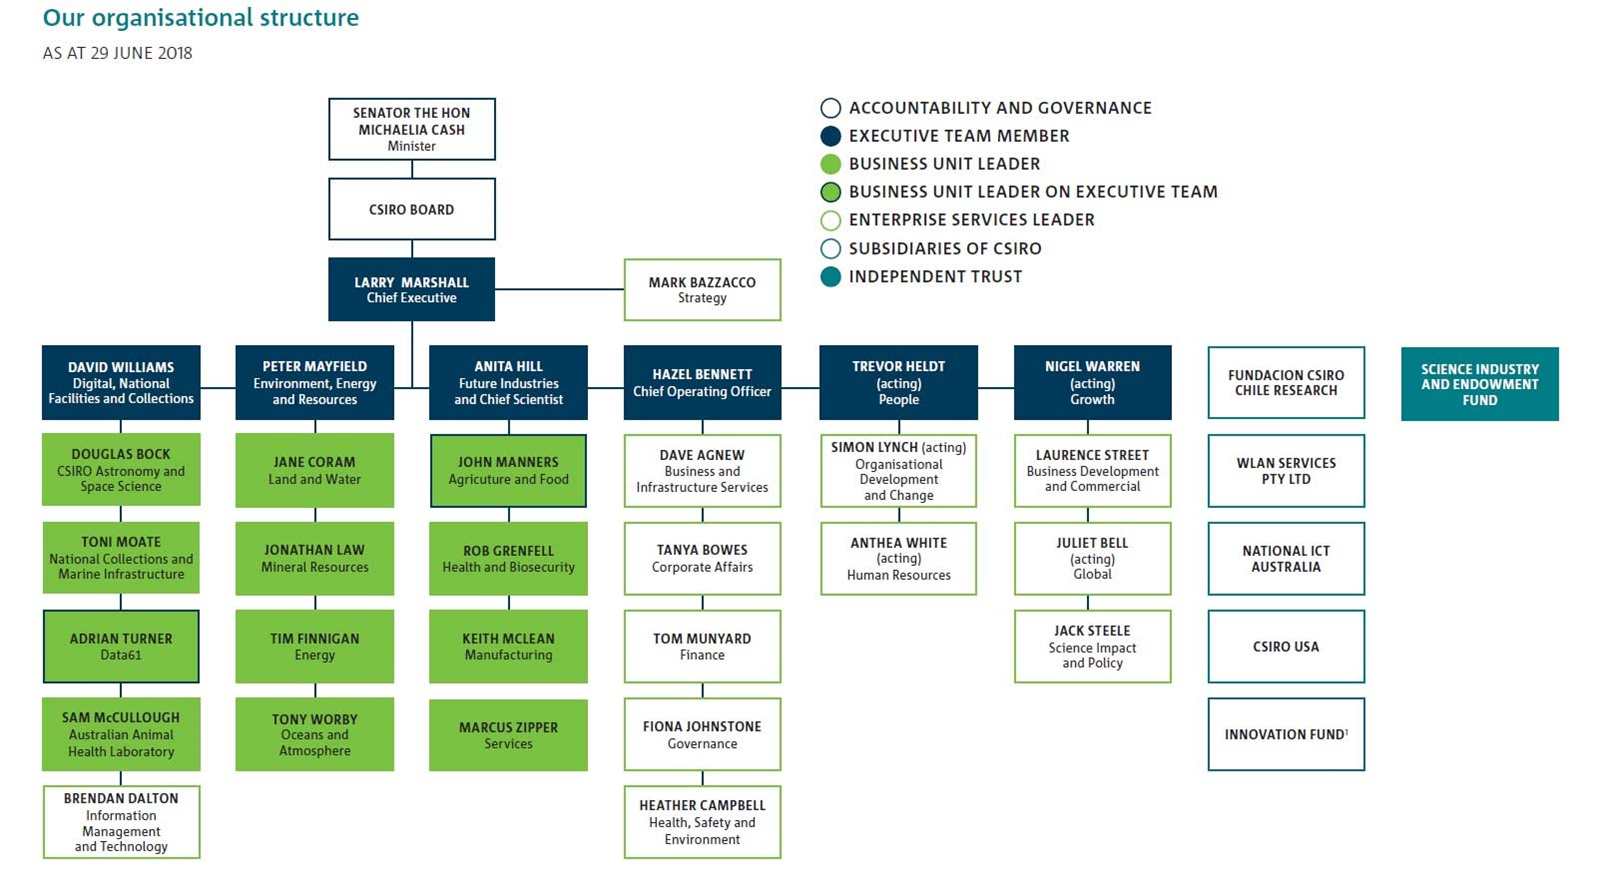
\includegraphics[width=16cm]{figures/csiro_struct.jpg}
    \caption{CSIRO Organizational Structure}\vspace{-4mm}
\end{figure}

\subsection{Areas of Interest}

\paragraph{}
DATA61 strives to build Australia's data driven future. Their programs can be divided into Analytics, Cyber-Physical Systems, Consumer Data Standards, Decision Sciences, Software and Computation Systems and Engineering and User Experience Design. Some of their key projects are:

\subsubsection*{Emesent - Hovermap}

\paragraph{}
Emesent is a spin-off company from the highly successful Hovermap project of DATA61. It is a state-of-the-art LiDAR based SLAM system to be fixed on industrial drones. Hovermap can be also be used to analyze the structure and composition of various mineral deposits in rock cliffs, map underground mines and caves and used in forensics to analyze crime scenes.

\subsubsection*{SLAM}
\subsubsection*{Legged Robots}
\subsubsection*{}

\subsection{Current Situation}

\paragraph{}
The RAG of CSIRO was recently selected as one of the six teams worldwide for the DARPA Subterranean Challenge by United States Department of Defense. Therefore the next four years of research in Robotics in CSIRO will be more focused on developing robots that can simultaneously map and navigate underground tunnels, caves and mines without GPS or reliable communication with humans. For this task, incorporating machine learning into the workflow of algorithm development and testing is of paramount importance for all researches in RAG. I addressed this problem by developing an efficient end-to-end pipeline for this and demonstrating it through two projects.

\subsection{Impacts on Sri Lankan Industry}

\subsection{SWOT Analysis}
\subsubsection{Strengths}
\subsubsection{Weaknesses}
\subsubsection{Opportunities}
\subsubsection{Threats}

\subsection{DARPA Subterranean Challenge}
\label{ssec:darpa}

%Image: Darpa challenge
\begin{figure}[H]
    \centering
    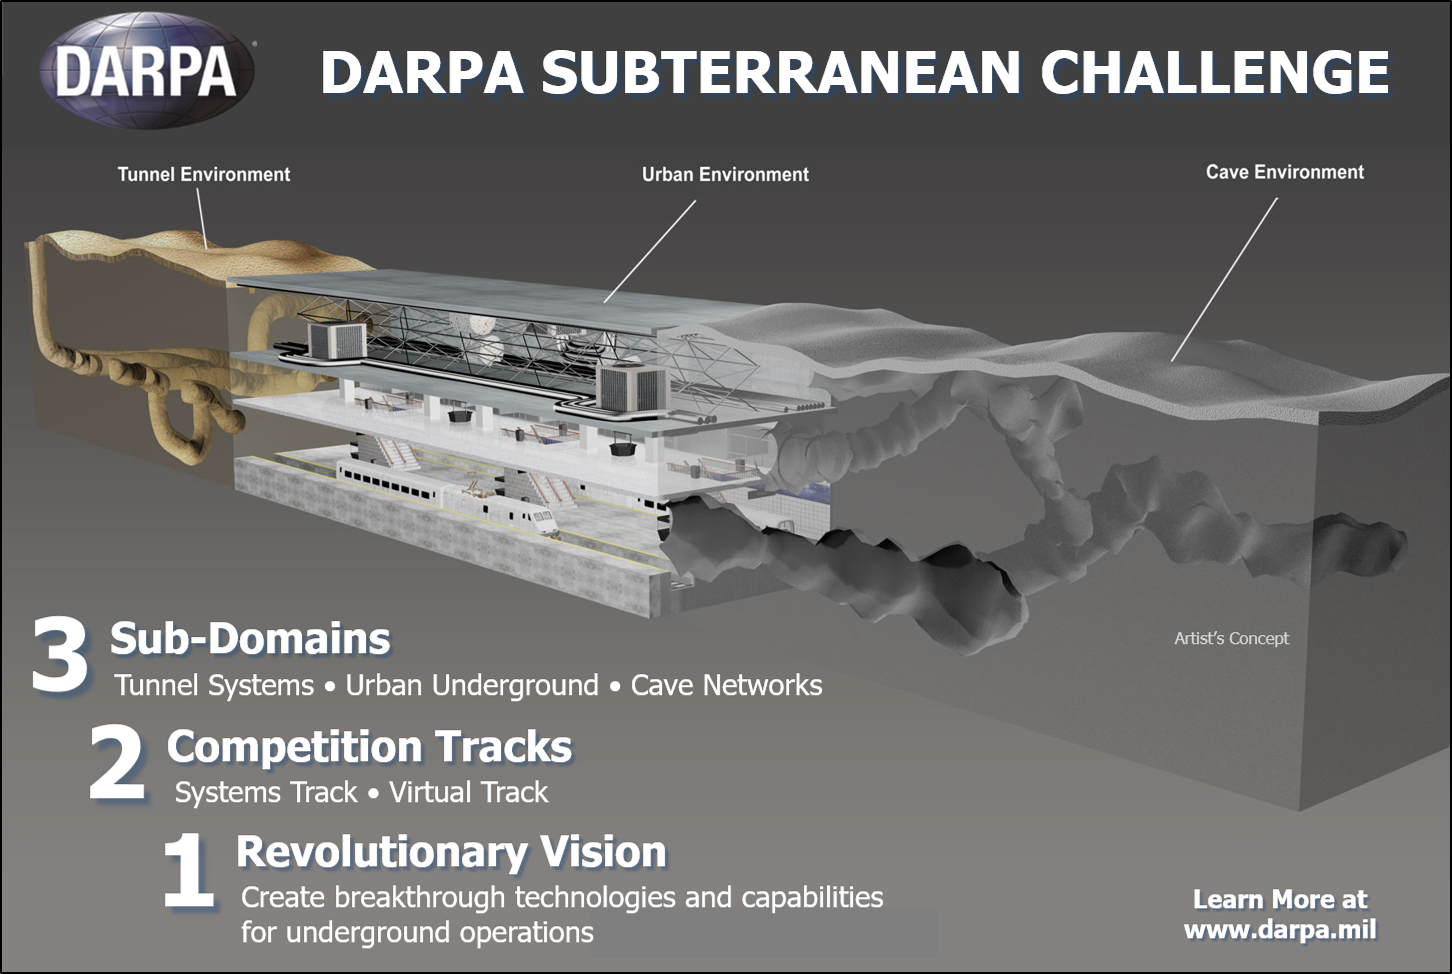
\includegraphics
        [width=15cm]
        {figures/subt_challenge.png}
    \caption{CSIRO focuses on DARPA challenge}\vspace{-4mm}
\end{figure}

\subsection{Usefulness to the Country}
\subsection{Suggestions to Improve the Company}